\documentclass{llncs}
\usepackage{llncsdoc}
\usepackage{epsfig}

%
\begin{document}
\def\addtocontents#1#2{}%
\def\addcontentsline#1#2#3{}%
\def\markboth#1#2{}%
%
%\title{PGR : A Programming package for Physics Processing Units Generation using an FPGA-Based System}
%\title {Towards Reconfigurable High Performance Computing for scientific many-body simulations}
%\title {PGR : A Software Package for Reconfigurable High Performance Computing}
\title {A Methodology for implementing Reconfigurable Physics Processing Units}

\author{Tsuyoshi Hamada\inst{1}, Naohito Nakasato\inst{1}}

\institute{Computational Astrophysics Group,\\
The Physical and Chemical Research Institute (RIKEN),\\
Wako, Saitama 351-0198, Japan}

\maketitle
%
\begin{abstract}
This paper describes a methodology for implementing FPGA-based
accelerator from a high-level specification in a small special-purpose
language.  The idea is to generate, from a high-level description, (a)
a suitable configuration file for the FPGAs, (b) the C source code for
interfacing with the FPGA-based processors that has been generated,
and (c) a software emulator. The FPGA configuration is build by
combining components from a library of parametrized arithmetic
modules; these modules implement fixed point, floating point and
logarithmic number system with flexible bitwidth and pipeline stages. To
prove our methodology to be correct, we developed PROGRAPE-3 system as
a target hardware platform and implemented $N$-body calculation
algorithm using PGR.  With the PROGRAPE-3 system of a minimum
composition, we have achieved peak performance of 162 Gflops and
mesured performance of 100 Gflops on actual numerical simulation.
In the FPGA-based high performance computing area,
our methodology and implementation is wonderful for all to others existed.
\end{abstract}
%
\section{Introduction}
%

Recently, scientific computation using FPGAs begins to be promising
and attract a several group of astrophysicists.
Previously, many works related to scientific computation using FPGAs
have been reported and, roughly speaking, 
those works can be classified into following three subjects;
(A) hardware implementations, (B) construction of arithmetic modules
and (C) programming technique for generating a
computing core for FPGAs. 
In this work, we present results of our current efforts
for each of those subjects. 
Specifically, we have constructed a software package specially 
tuned for accelerating scientific computations with FPGA-based systems.
Although we will show details of our methodology in the following sections, 
first we briefly describe each subject as follows.

(A) {\bf Hardware Implementations}:
In the first subject of hardware implementations,
PROGRAPE-1(PROgrammable GRAPE-1)\cite{HFKM00} is
an earliest example of the use of a reconfigurable hardware for
scientific computation.  PROGRAPE-1 is an FPGA-Based Accelerator(FBA)
for astrophysical many-body simulations. It is implemented with two
Altera EPF10K100 FPGAs. Comparing with modern FPGAs, the EPF10K100 is
old-fashioned and has only 100k gates per one chip.
On the PROGRAPE-1 board, they have implemented a computing core
that calculates gravitational force
$\mathbf{a}_i$ of $i$-th particle exerted by all other particles
used in astrophysical many-body simulations:
\begin{equation}
\mathbf{ a}_i = \sum_j a_{ij} = \sum_j {m_j \mathbf{ r}_{ij} \over (r_{ij}^2 + \varepsilon^2)^{3/2}}
\end{equation}
where $\mathbf{r}_{ij}$ is a distance between $i$ and $j$-th particles
($\mathbf{r}_j - \mathbf{r}_i $), 
$m_{j}$ is mass of $j$-th particle, and $\varepsilon$ is a softening parameter
that prevents a zero-division.
They have obtained peak throughput performance of 0.96 Gflops
for this calculation.
An essential point of the PROGRAPE-1 is using fixed point and short-length
logarithmic number formats instead of the IEEE standard floating point (FP) format. 
In the processor core of PROGRAPE-1, they have adopted 
20-bit fixed point format in a first stage for subtraction,
14-bit logarithmic number format(7-bit exponent,
5-bit mantissa, sign flag and non-zero flag)
in inner stages for division and square root etc., 
and 56-bit fixed point format in a last stage for summation.
That is though available resource of FPGA systems is limited,
FBA systems can be attractive and competitive if an application does
not need high accuracy such as double precision accuracy 
that is used in general comporting with conventional CPUs.
After the PROGRAPE-1, a several group have reported
similar FBA systems (\cite{LKM02}\cite{SS03}\cite{AKEDC04}).
In all of those works, they have used HDL as system programming language
for constructing a computing core and
mentioned the need of automation the task of programming.
We will show our answer to such demands in this paper.
To prove our methodology described in this paper to be correct,
we have developed new FBA board (PROGRAPE-3 board) with modern FPGAs.
as a target hardware.

(B) {\bf Arithmetic Modules}:
In the second subject, main task is to construct a library
of parametrized FP format and other format arithmetic modules (AM). 
For example, \cite{JL01}\cite{LCCN03} have presented parametrized FP adders and
multipliers, and \cite{LKM02}\cite{WN04} presented parametrized FP square-roots and divisions. 
However, even if these basic AMs are existed, 
it is insufficient to construct a computing core for scientific computations.
In most of those works, square root and divisions are implemented
using subtracters and shifters. 
This approach is not suitable especially in pipelined data-path,
because the carry propagation of ripple-carried subtracter becomes long.
Increasing carry propagation is a fatal problem even for modern FPGAs.
Instead of using those standard algorithm, 
implementing Function Evaluation Units(FEUs) is a possible alternative approach.
One can use FEUs for calculating arbitrary functions such as
$\sqrt{x}$, $log(x)$, ${\rm exp}(x)$ that are commonly appeared in 
scientific computations.
In implementing a FEU, one can have three approxmation methods such as
a table look-up method ($0-$th order), a polynomial approximation method ($n-$th order),
or the hybrid method\cite{FO01}\cite{M97}. 
With HDLs that is static in its nature except generic parameters
such as \verb|GENERIC| or \verb|ATTRIBUTE|,
implementation of a general FUE that support arbitrary functions, 
different methods, and variable precision is highly difficult task.
To solve this problem, one can construct a software that dynamically generate 
HDL descripton for a FEU.
The approach of dynamic generation is applicable for generating
not only FEUs but general FP-AMs that is also
better to support variable precisions.
Here in this work, we have constructed such software for our purpose.
At run-time, by selecting a disired functions and an approxmation method
(in case of the FEU generation) or desired precision and numberd format
(in case of the AM generation), our software generate a corresponding module.
Details will be described in Section 2.1.

(C) {\bf Generation of a Computing Core}:
Even if the FP-AMs are existed as libraries or generated
from a software, one needs a deep understanding of details of such AMs
to construct a computing core for the purpose.
The task in the third subject is to solve the those issues
of generating a computing core using the AMs.
A real concern here is how to convert a scientific application
written in a high-level language such as C, Java or C++ into a FPGA configuration.

PAM-Blox\cite{MMF97} and JHDL\cite{BH98} are first examples
to allow such conversion from C++ and Java, respectively.
The PAM-Blox concentrates on automation and simplicity to explore the design space.
The JHDL treats circuits as objects and but has only a few elemental FP-AMs
so that it seems not to be interested in scientific computations so much.  
In both work, authors have emphasized the importance of automatic
generation of APIs that is needed to communicate between FBAs and a host processor.
In general, an software between the FBA and the host processor
should be implemented to maximize data transfer rate and minimize latency.
Even if a smart tool can generates an FPGA configuration of a computing core,
one can't necessarily write such high performance communication software.

As well as communication software, 
the performance of a particular application
is very sensitive to detailed {\it architecture} of a computing core.
Here, we consider a computing core consists of inner and outer core.
Specifically, in astrophysical many-body simulations,
one can think an inner core is a calculation unit of gravitational force between two particles
shown in eq. (1) and an outer core is a memory unit that feeds data of two particles 
to the inner core and fetch results from the inner core. 
An obvious implantation of this core is that the outer core
feeds position and mass of each $i-$th and $j-$th particles and
and fetch partial force $a_{ij}$ in each step of the summation.
This implementation is most flexible but worst efficient in terms of data transfer.
In the PROGRAPE-1 (and other family of GRAPE\cite{MT98}),
the computing core is implemented such that
(a) data of $i-$th particle is stored inside the inner core
(b) the inner core accumulate partial sums inside
and (c) the outer core feeds $j-$th continuously and 
fetch only the accumulated force $a_{i}$.
Clearly, even with a same inner core, performance 
can change drastically depending on detailed {\it memory architecture} of a outer core.

In the PAM-Blox\cite{MMF97}, authors have introduced an important concept
of {\it domain specific compiler} \cite{MPMF01}. 
In the domain specific compiler, the promising application is limited by
compiler. The point is that there is no almighty architecture for any problem
and we sympathize with their ideas very much as already mentioned.
Specifying the application domain produces good results for
the tool developer and the tool users.  For the tool developer, the
language specification becomes compact so it can be easy to implement
a compiler that specializes to an application domain if once the
module generator has been completed as a core component of a
programming tool.  For the tool users, it becomes clear whether the
tool agrees with a purpose and easy to understand such a compact
language specification.
Because PAM-Blox seems very wonderful tool, we feel they might appeal
more positively and very regrettable not to try to accelerate 
scientific computations such as gravitational many-body simulations.

In this paper, we have adopted the above memory
architecture of the GRAPE family (schematical example shown in figure \ref{fig4}).
That is a problem domain of our software package
that we are developing so far is a particle-based simulation.
Our developing software, 
Processors Generator for Reconfigurable system (PGR system),
analyzes a description of a computing core
written in the PGR Description Language (PGDL; descrived in Section 2.4)
as input and then generates necessary hardware descriptions in HDL,
a bit-level emulator, and communication softwares automatically.
Note the generated hardware descriptions should be synthesized by a CAD software
and one can obtain FPGA configuration data of the computing core. 

In the following sections, we describe details of our
newly developed parametrized AMs that are key components of the PGR package
and show a simple design example using the PGDL.
Moreover, in section 3, we present an example of a real application 
and show obtained performance on the PROGRAPE-3 board.
Finally, we summarize our results in section 4.
%
\section{PGR : Processors Generator for Reconfigurable systems}
\subsection{PgModules : PGR Parametrized Arithmetic Modules}

PgModules(PGR parametrized arithmetic modules) implement fixed point, 
FP and logarithmic number system (LNS) AMs and 
are the most low-level components for the PGR package.
These moduels include addition, subtraction, multiplication, division, and square-root, etc. 
Currently, the PGR package supports
29 parametrized AMs as shown in table \ref{tabpgmod}.

In this table, modules with {\tt pg\_float} correspond to FP arithmetics.
We define internal FP format such that 1-bit for a sign, 
1-bit for a non-zero expression, $n$-bit for exponent, 
and $m$-bit for mantissa, where $m$ and $n$ can be 
changed arbitrary up to 23 and 8, respectively.
For example, in the PGDL, we can generate a float-point addition module
as follows;
\begin{verbatim}
pg_float_add(x,y,z,26,16,1);
\end{verbatim}
Here, the arguments are the first input, the second input, output,
total bit-length of FP format, bit-length for mantissa,
and number of pipeline stages, respectively, from the first to sixth argument.
This example calculates
$z = x + y$, where $x,y,z$ are 26-bit FP numbers and mantissa is 16-bit.
And a number of pipeline stage for this arithmetic is one.
Note that for the rounding operation, we have implemented nine types
of several options that also can be changed by a hidden argument in the PGDL.
If this argument is omitted like above example, 
a rounding to the nearest even is selected.

\begin{table}
  \begin{center}
    \caption{a list of PgModules}

    \begin{minipage}{.45\linewidth}
      \begin{tabular}{ll}
	\hline
	floating point format & \\
	\hline
	    {\tt pg\_float\_add}           &  $+$\\
	    {\tt pg\_float\_unsigned\_add} &  $+$\\
	    {\tt pg\_float\_sub}           &  $-$\\
	    {\tt pg\_float\_unsigned\_sub} &  $-$\\
	    {\tt pg\_float\_mult}          &  $\times$\\
	    {\tt pg\_float\_div}           &  $/$ \\
	    {\tt pg\_float\_sqrt}          &  $\sqrt{x}$ \\
	    {\tt pg\_float\_square}        &  $x^2$\\
	    {\tt pg\_float\_recipro}       &  $x^{-1}$\\
	    {\tt pg\_float\_expadd}        &  $x \cdot 2^{N}$\\
	    {\tt pg\_float\_negate}        &  $-x$\\
	    {\tt pg\_float\_compare}       &  $==$\\
	    {\tt pg\_float\_compare\_abs}  &  $==$\\
	    {\tt pg\_float\_compz}         &  $>0$\\
	    {\tt pg\_float\_compz\_abs}    &  $>0$\\
	    {\tt pg\_float\_accum}         &  $+=$\\
	    {\tt pg\_float\_unsigned\_accum}& $+=$\\
	    {\tt pg\_float\_fixaccum}      &  $+=$\\
	    \hline
      \end{tabular}
    \end{minipage}
    \hspace{2.3pc}
    \begin{minipage}{.45\linewidth}
      \begin{tabular}{ll}
	\hline
	fixed point format & \\
	\hline
	{\tt pg\_fix\_addsub}          &  $+$, $-$\\
	{\tt pg\_fix\_mult}            &  $\times$\\
	{\tt pg\_fix\_unsigned\_mult}  &  $\times$ (unsigned)\\
	{\tt pg\_fix\_accum}           &  accumulate\\
	\hline
	LNS format& \\
	\hline
	{\tt pg\_log\_add}             &  $+$\\
	{\tt pg\_log\_unsigned\_add}   &  $+$ (unsigned)\\
	{\tt pg\_log\_muldiv}          &  $\times$, $/$\\
	{\tt pg\_log\_shift}           &  $\sqrt{x}$, $x^2$\\
	\hline
	format conversion & \\
	\hline
	{\tt pg\_conv\_fixtofloat}     &  fix $\Rightarrow$ float\\
	{\tt pg\_conv\_floattofix}     &  float $\Rightarrow$ fix\\
	{\tt pg\_conv\_ftol}           &  fix $\Rightarrow$ log\\
	{\tt pg\_conv\_ltof}           &  log $\Rightarrow$ fix\\
	\hline
      \end{tabular}
    \end{minipage}
  \end{center}
  \label{tabpgmod}
\end{table}

Modules {\tt pg\_fix\_addsub} and {\tt
pg\_fix\_accum} are fixed point format adder/subtracter and
accumulator, respectively.  Modules {\tt pg\_log\_muldiv} and {\tt
pg\_log\_unsigned\_add} are LNS multiplier/divider and
unsigned adder, respectively.
In the LNS, a positive,
non-zero real number $x$ is represented by its base-2 logarithm $y$ as
$x=2^{y}$.
This LNS is useful because operation such as multiplication and square root
are easier to implement than in the usual FP format.
For more details of the LNS, see GRAPE-5 paper
\cite{KFMT00}.
Module {\tt pg\_log\_shift} is an LNS shifter.
Shift operations in the LNS corresponds to
square (left shift) and squared root (right shift). 

Modules with {\tt pg\_conv} are converters from a particular format
into another format, e.g., {\tt pg\_conv\_floattofix} converts
a FP number into a corresponding fixed point number.

In tables \ref{tabpg_float_unsigned_add},
\ref{tabpg_float_sqrt}, \ref{tabpg_float_recipro},
\ref{tabpg_log_unsigned_add}, we show
resource consumption and clock frequency of several important
parametrized arithmetic modules.
Despite we have implemented all of the parametrized AMs
from full scratch, the obtained performance results
are as same as other implementations such as Manheim's (\cite{LKM02}).

\begin{table}
  \begin{center}
    \begin{minipage}{.45\linewidth}
      \caption{Multiplier(floating point)}
      \begin{center}
	\begin{tabular}{cccrr}
	  \hline
	  length  & length(mantissa) & stages & MHz & slices\\
	  \hline
	  18   &  9 & 2 & 290.192 &  31 \\
	  &    & 0 & 133.387 &  15 \\
	  \hline
	  26   & 17 & 4 & 224.266 &  56 \\
	  &    & 2 & 151.953 &  41 \\
	  &    & 0 &  80.762 &  23 \\
	  \hline
	  33   & 24 & 3 & 136.986 &  93 \\
	  &    & 0 &  68.847 &  56\\
	  \hline
	\end{tabular}
      \end{center}
      \label{tabpg_float_mult}
    \end{minipage}
    \hspace{2.4pc}
    \begin{minipage}{.45\linewidth}
      \caption{Multiplier(floating point)}
      \begin{center}
	\begin{tabular}{cccrr}
	  \hline
	  length  & length(mantissa) & stages & MHz & slices\\
	  \hline
	  18   &  9 & 2 & 290.192 &  31 \\
	  &    & 0 & 133.387 &  15 \\
	  \hline
	  26   & 17 & 4 & 224.266 &  56 \\
	  &    & 2 & 151.953 &  41 \\
	  &    & 0 &  80.762 &  23 \\
	  \hline
	  33   & 24 & 3 & 136.986 &  93 \\
	  &    & 0 &  68.847 &  56\\
	  \hline
	\end{tabular}
      \end{center}
      \label{tabpg_float_mult}
    \end{minipage}
  \end{center}

  \begin{center}
    \begin{minipage}{.45\linewidth}
      \caption{Square root (floating point)}
      \begin{center}
	\begin{tabular}{cccrr}
	  \hline
	  length  & length(mantissa) & stages & MHz & slices\\
	  \hline
	  18   &  9 & 4 & 215.517 & 86 \\
	  &    & 2 & 157.754 & 71 \\
	  &    & 0 &  79.971 & 51 \\
	  \hline
	  26   & 17 & 4 & 188.964 & 140 \\
	  &    & 2 & 127.959 & 116 \\
	  &    & 0 &  56.500 &  84 \\
	  \hline
	  33   & 24 & 5 & 141.243 & 425 \\
	  &    & 3 & 104.998 & 392 \\
	  &    & 1 &  70.210 & 374 \\
	  \hline
	\end{tabular}
      \end{center}
      \label{tabpg_float_sqrt}
    \end{minipage}
    \hspace{2.4pc}
    \begin{minipage}{.45\linewidth}
      \caption{Adder (LNS)}
      \begin{center}
	\begin{tabular}{cccrr}
	  \hline
	  length  & length(mantissa) & stages & MHz & slices\\
	  \hline
	  14   &  6 & 4 & 201.077 & 94 \\
	  &    & 2 & 151.207 & 73 \\
	  &    & 0 &  64.545 & 57 \\
	  \hline
	  17   &  9 & 5 & 195.369 & 116 \\
	  &    & 2 & 138.042 &  92 \\
	  &    & 0 &  58.828 &  86 \\
	  \hline
	  20   & 12 & 6 & 218.293 & 191 \\
	  &    & 2 & 135.125 & 123 \\
	  &    & 0 &  53.562 & 115 \\
	  \hline
	\end{tabular}
      \end{center}
      \label{tabpg_log_unsigned_add}
    \end{minipage}
  \end{center}
\end{table}

\subsection{PGR five layers model}
To make the PGR software system independent on a specific hardware,
we create the PGR five layers model which divide 
an FBA into five parts.
Figure \ref{fig5model} shows the PGR five layers model, 
and it's composed of User Program Layer(UPL), API Layer(APL),
Device Driver Layer(DDL), I/O \& Control Logic Layer(ICL) and
Arithmetic Logic Layer(ALL).

The UPL is a user application which communicates with an FBA through the APL.
The APL contains the top level API implementations that
doesn't depend on an individual FBA.
The DDL consists of both a low level communication library and a device driver software. 
The ICL is a glue logic such as the PCI interface logic and 
local I/O logic on an FBA.
The ALL corresponds to a {\it computing core} explained in Section 1
and is composed of AMs and control logics.

\begin{figure}[htb]
\begin{center}
  \begin{minipage}{.45\linewidth}
    \begin{center}
    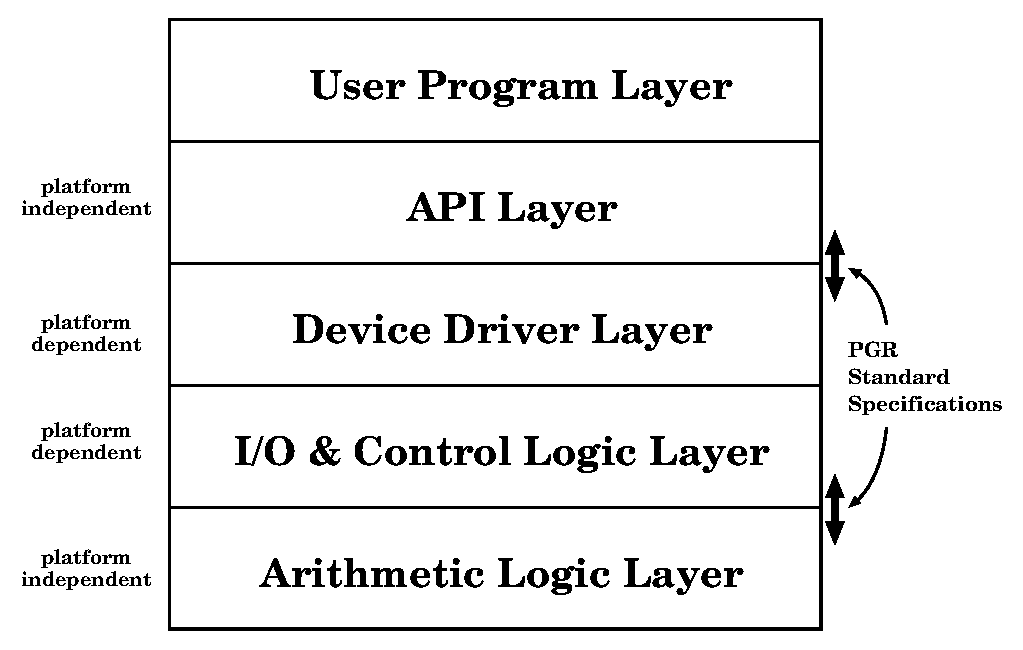
\includegraphics[angle=+0, width=1.2 \linewidth]{./mat/5model.eps}
    \caption{PGR five layers model.}
    \label{fig5model}
    \end{center}
  \end{minipage}
  \hspace{2.4pc}
  \begin{minipage}{.45\linewidth}
    \begin{center}
    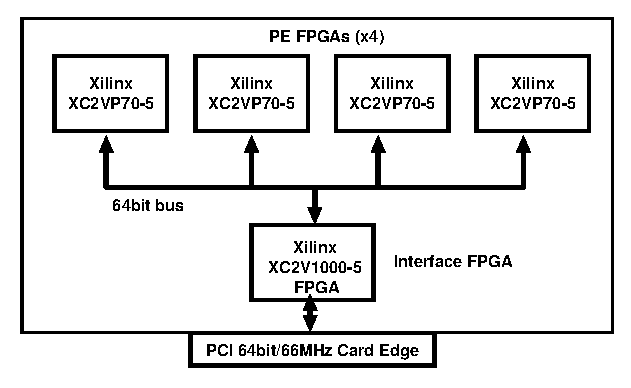
\includegraphics[angle=+0,width=1.2 \linewidth]{./mat/pg3.eps}
    \caption{PROGRAPE-3 board structure}
    \end{center}
  \end{minipage}
\end{center}
\end{figure}

\subsection{PGDL: PGR Description Language}
In this subsection, we illustrate how pipeline processors(or computing cores)
are described in the PGDL and how such description is converted 
into HDL sources for pipelined processors.

\begin{figure}[htb]
\begin{center}
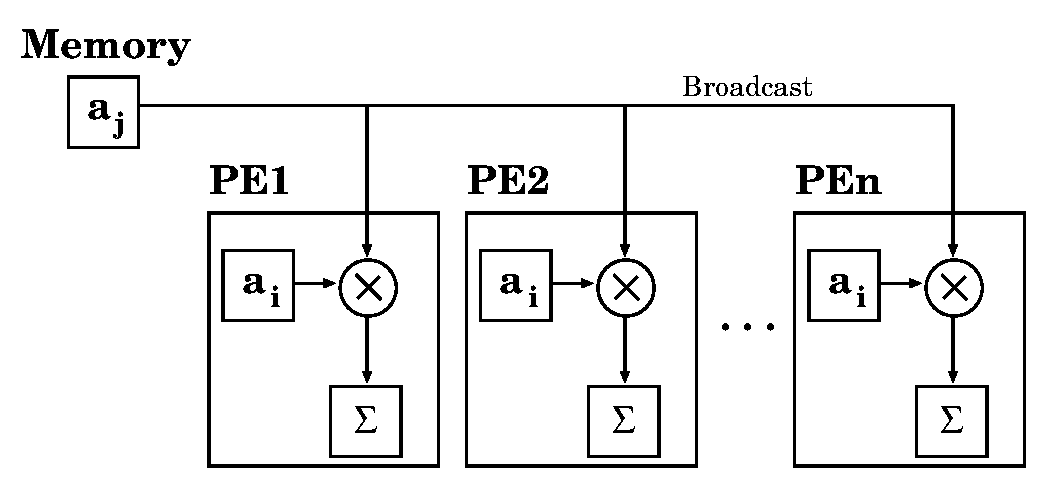
\includegraphics[angle=+0,width=8cm]{./mat/simple.eps}
\caption{Block diagram of the example processors(PEs).}
\label{fig4}
\end{center}
\end{figure}

With the current version of the PGR package, 
it is specially tuned to generate pipelined processors
for particle-besed simulations as explained already.
It is expressed as the following summation form;
\begin{equation}
f_i = \sum_{j = 1}^{n} F(\boldmath{p}_i, \boldmath{p}_j),
\end{equation}
where $f_i$ is summation for $i$-th data, $\boldmath{p}_i$ are
some values associated with $i$-th data, and
$F$ expresses calculations where $i$-th and $j$-th data are as inputs.

As an example target, we consider the following artificial calculations;
\begin{equation}
f_i = \sum_j^n {a_i a_j}.\qquad (i=1,...,n)
\end{equation}
Figure \ref{fig4} shows the block diagram for this example.
Here, $a_i$ and $a_j$ are scalar values for $i$-th and
$j$-th elements, respectively.
This target simply calculates a product of $a_i$ and $a_j$, 
and sums the product up for all $j$.

Figure \ref{fig5} shows the PGDL description of this target function.
In this example, one already sees essential ingredients of an FBA:
data, their representation, functional form of arithmetic operations
between data $i$ and $j$.
The first two lines define the bit-length of the FP format.
These definitions are actually used in the next block
(three lines starting with ``/''),
which defines the register and memory layout,
which also determine the interface API etc. 
For the data $a_i$ (and $a_j$), we use a FP format,
with 26 bits in total (1-bit for sign, 1-bit for non-zero flag, 8-bits
for exponent, and 16-bits for mantissa).
The line ``/NPIPE'' specifies a number pipeline processors (10 processors in this case).
The final part describes the target function itself using
parametrized AMs. It has C-like appearance, but
actually defines the hardware modules and their interconnection.

From such PGDL description, the following ALL (as shown in figure \ref{fig4})
is generated; the $i$-th data is stored in the on-chip memory,
and new data ($j$-th data) is supplied at each clock cycle.
The $i$-th data is unchanged during one calculation, and 
the result ($f_i$) is stored in the register.

\begin{figure}
\scriptsize
\begin{verbatim}
#define NFLO 26
#define NMAN 16

/JPSET x,  aj[], float, NFLO, NMAN;
/IPSET y,  ai[], float, NFLO, NMAN;
/FOSET z,  fi[], float, NFLO, NMAN;

/NPIPE 10;

pg_float_mult      (x,   y,  xy, NFLO, NMAN, 1);
pg_float_accum     (xy,  z,      NFLO, NMAN, 1);
\end{verbatim}
\caption{An example of design entry file written in PGDL}
\label{fig5}
\end{figure}

\section{Application}
To show the possibility of the PGR package, we have implemented gravitational
force (as shown in eq. (1)) pipeline for astrophysical many-body simulations
Figure \ref{figgravfloat_pgdl} and \ref{figgrav5_pgdl}
show PGDL descriptions for this gravitational force pipeline
using 26-bit FP operations and 17-bit LNS operations, respectively.
Note there are a several differences between two descriptions.
To test our FP and LNS modules are really correct, 
we have generated gravity pipelines with a several different precisions
and compared results with the results obtained by double-precision FP
calculations in Figure \ref{SrError}.




Figure \ref{fig_grav_float_delay} shows a generated 
data flow graph that corresponds to the FP pipeline.
Since all operations must be synchronized in pipeline processors, 
a module in the PGR package automatically inserts
delay register, which are indicated by bold solid circles,
for synchronization.

In Figure \ref{SrError}, we compare results for

offorce error of our 


We note that a similar package to the PGR system have been reported in \cite{THYL04}.
The CAST(Computer Arithmetic Synthesis Tool) is a tool
for implementing astrophysical many-body simulations.
The main concern about CAST is that the CAST only generate
a computing core and they doesn't take account for API generation. 
In general numerical calculations with reduced-length arithmetic, 
type conversions and scaling operations are confusing and
an implementation of APIs becomes troublesome inevitably.
And as we thought, they seemed to be making serious mistakes in their result.
In their figure 12a, the 8-bit precision of their FP
implementation is not better accurate than the GRAPE-3 which uses 5-bit precision.
Such inconsistencies seem to be due to by mistakes of scaling.
Let us add a few more words for their honor, their modules may be good
in accuracy but the implementation of APIs are wrong. 
On the other hand, using the PGR system, possible users, 
who want to accelerate their particle simulations with an FBA,
can concentrate on writing their application in the PGDL.
This means that the PGR system can drastically reduce the amount of
the work (and needed knowledge) of such user.
More importantly, the PGDL does not depends on a specific hardware
(e.g., PROGRAPE-3) and this make it possible to
reuse a application written in the PGDL on a newly developed FBA
when the PGR package supports the new FBA.




\subsection{Real Performance}



For each FP and LNS pipelines, one pipeline comsumes XXX and XXX slices, respectively.

In Figure 








\section{Discussion}



On the real hardware (PROGRAPE-3 board in the present work), 
24 FP and 64 LNS pipelines have been correctly working in parallel at 66.6MHz.
Here, {\it correctly working} means that gravity force calculated by
the PROGRAPE-3 board for $8192$ particles is exaxcly same with results
obtained by software emulator.
In table \ref{tabcompg5}, we compare those two implementations
with the GRAPE-5 system\cite{KFMT00}
(actually, the LNS piplines is actually equivalent to the GRAPE-5).
For each implementations, the peak throughput performance 
of single PROGRAPE-3 board is 60.8 Gflops and 162.1 Gflops, respectively.
Here, the number of floating-point operations per one interaction is 38.
The peak performance of the LNS pipelines on single PROGRAPE-3
board is five times faster than one GRAPE-5 board.
And even if we use twice the accuracy (i.e., FP pipelines),
the performance is the still two times better than the GRAPE-5.

Finally, figure \ref{MESURE-PERFORM} shows the mesured calculation speed of
single PROGRAPE-3 board with the LNS implementation as a function of 
number of particles $N$. Here, we show the results for the direct-summation algorithm.
Because the order of the calculation and communication is $O(N^2)$ and $O(N)$
respectively, the mesured speed approaches the peak speed as the
number of particles increases.

\begin{figure}
\scriptsize
{\tiny
\begin{verbatim}
 1 /* -------------------------------------------------- MACRO */
 2 #define NFLO 26
 3 #define NMAN 16
 4 #define NFIX 57
 5 #define NACC 64
 6 #define FOFFSET (131072.0)
 7 #define NST_MULT 2
 8 /* ----------------------------------------- I/O DEFINITION */
 9 /JPSET xj[3], x[][],  float, NFLO, NMAN;
10 /JPSET mj,    m[],    float, NFLO, NMAN;
11 /IPSET xi[3], x[][],  float, NFLO, NMAN;
12 /IPSET ieps2, eps2,   float, NFLO, NMAN;
13 /FOSET sx[3], a[][],  fix,   NACC, (-1.0/FOFFSET);
14 /CONST_FLOAT fofst, FOFFSET, NFLO, NMAN;
15
16 /NPIPE 6;
17 /* ------------------------------------------- PE DATA FLOW */
18 pg_float_sub(xi,xj,   dx,  NFLO,NMAN,4);
19 pg_float_mult(dx,dx, dx2,           NFLO,NMAN, NST_MULT);
20 pg_float_unsigned_add(dx2[0],dx2[1], x2y2,  NFLO,NMAN,4);
21 pg_float_unsigned_add(dx2[2],ieps2,  z2e2,  NFLO,NMAN,4);
22 pg_float_unsigned_add(x2y2,z2e2,r2, NFLO,NMAN, 4);// x2y2+z2e2
23 pg_float_sqrt(r2,r1,       NFLO,NMAN, 3);        // sqrt(r2)
24 pg_float_recipro(r1,r1i ,  NFLO,NMAN, 2);        // 1/r1
25 pg_float_mult(r1i,r1i,r2i, NFLO,NMAN, NST_MULT); // r1i * r1i
26 pg_float_mult(r1i,r2i,r3i, NFLO,NMAN, NST_MULT); // r1i * r2i
27 pg_float_mult(r3i,mj,mf,   NFLO,NMAN, NST_MULT); // r3i * mj
28 pg_float_mult(mf,fofst,mfo,NFLO,NMAN, NST_MULT); // mf  * fofst
29 pg_float_mult(mfo,dx,fx,   NFLO,NMAN, NST_MULT); // mfo * dx[]
30 pg_conv_floattofix(fx,ffx, NFLO,NMAN,NFIX,1); // fxo[] -> ffx[]
31 pg_fix_accum(ffx,sx,       NFIX, NACC, 4);    // sx[] += ffx[]
\end{verbatim}
}
\caption{a PGDL for gravitational force calculation (using 26-bit floating point arithmetics)}
\label{figgravfloat_pgdl}
\end{figure}

\begin{figure}
\scriptsize
{\tiny
\begin{verbatim}
 1 /* -------------------------------------------------- MACRO */
 2 #define NPOS 32
 3 #define NLOG 17
 4 #define NMAN 8
 5 #define NCUT 6
 6 #define NFOR 57
 7 #define NACC 64
 8 #define xsize (100.0)
 9 #define mmin (1.220703125e-04)
10 #define xoffset (xsize/2.0)
11 #define xscale (pow(2.0,(double)NPOS)/xsize)
12 #define mscale (pow(2.0,95.38)/mmin)
13 #define escale (xscale*xscale)
14 #define foffset (pow(2.0,23.0))
15 #define fscale (-xscale*xscale*foffset/mscale)
16 /* ----------------------------------------- I/O DEFINITION */
17 /NPIPE 17;
18
19 /JPSET xj[3], x[][], ufix,      NPOS,xscale,xoffset;
20 /JPSET mj,    m[],   log,       NLOG,NMAN,mscale;
21 /IPSET xi[3], x[][], ufix,      NPOS,xscale,xoffset;
22 /IPSET ieps2, eps2,  log,       NLOG,NMAN,escale;
23 /FOSET sx[3], a[][], fix,       NACC,fscale;
24 /CONST_LOG fx_ofst,  8388608.0, NLOG, NMAN, 1.0;
25 /* ------------------------------------------- PE DATA FLOW */
26 pg_fix_addsub(SUB,xi,xj,xij,NPOS, 1);
27 pg_conv_ftol(xij,dx,NPOS,NLOG,NMAN, 2);
28 pg_log_shift(1,dx,x2,NLOG);
29 pg_log_unsigned_add_itp(x2[0],x2[1], x2y2,   NLOG,NMAN,4, NCUT);
30 pg_log_unsigned_add_itp(x2[2],ieps2, z2e2,   NLOG,NMAN,4, NCUT);
31 pg_log_unsigned_add_itp(x2y2,z2e2,   r2,     NLOG,NMAN,4, NCUT);
32 pg_log_shift(-1,r2,       r1,        NLOG);
33 pg_log_muldiv(MUL,r2,r1,  r3,        NLOG,1);
34 pg_log_muldiv(DIV,mj,r3,  mf,        NLOG,1);
35 pg_log_muldiv(MUL,mf,dx,  fx,        NLOG,1);
36 pg_log_muldiv(SDIV,fx,fx_ofst, fxo,  NLOG,1);
37 pg_conv_ltof(fxo,  ffx,              NLOG,NMAN,NFOR,2);
38 pg_fix_accum(ffx,  sx,               NFOR,NACC,1);
\end{verbatim}
}
\caption{a PGDL for gravitational force calculation (using 17-bit LNS)}
\label{figgrav5_pgdl}
\end{figure}

\begin{figure}[htb]
\begin{center}
\includegraphics[angle=+0,width=8cm]{./mat/grav_float_nodelay.eps}
\caption{Simple data flow of gravitational force pipeline.}
\label{fig_grav_float_nodelay}
\end{center}
\end{figure}

\begin{figure}[htb]
\begin{center}
\includegraphics[angle=+0,width=8cm]{./mat/grav_float_delay.eps}
\caption{Delay inserted data flow of gravitational force pipeline.}
\label{fig_grav_float_delay}
\end{center}
\end{figure}


\begin{table*}
\caption{Implementation result and comparison with other implementation}
\begin{center}
\begin{tabular}{lccc}
\hline
\hline
                     & GRAPE-5 board(8 ASICs) & \multicolumn{2}{c}{PROGRAPE-3 board(4 FPGAs)}  \\
\hline
format :input        & 32-bit FIX          & 26-bit FIX   & 32-bit FIX \\
format :internal     & 17-bit LNS          & 26-bit FP    & 17-bit LNS \\
format :accumulation & 64-bit FIX          & 64-bit FIX   & 64-bit FIX \\
A number of PEs      & 16                  &   24         &   64         \\
perk performance(Gflops)    & 48.6         & 60.8         & 162.1        \\
pair-wise error             & 10$^{-2.4}$   &  10$^{-4.8}$ & 10$^{-2.4}$ \\

\hline
\hline
\end{tabular}
\end{center}
\label{tabcompg5}
\end{table*}

\begin{figure}[htb]
\begin{center}
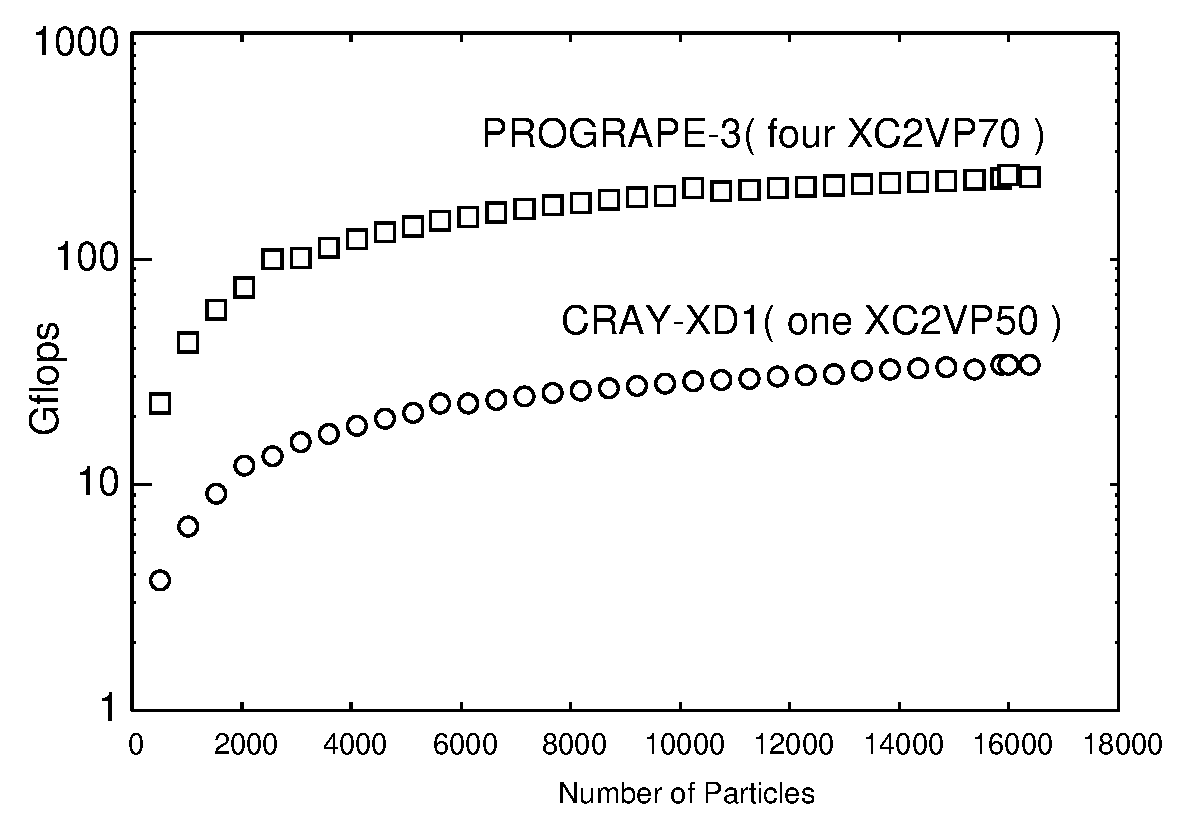
\includegraphics[angle=+0,width=8cm]{./mat/perform/graph.eps}
\caption{The mesured caluclation speed of single PROGRAPE-3 board in Gflops for the direct-summation algorithm, plotted as functions of the number of particles, N.}
\label{MESURE-PERFORM}
\end{center}
\end{figure}

\begin{figure}[htb]
\begin{center}
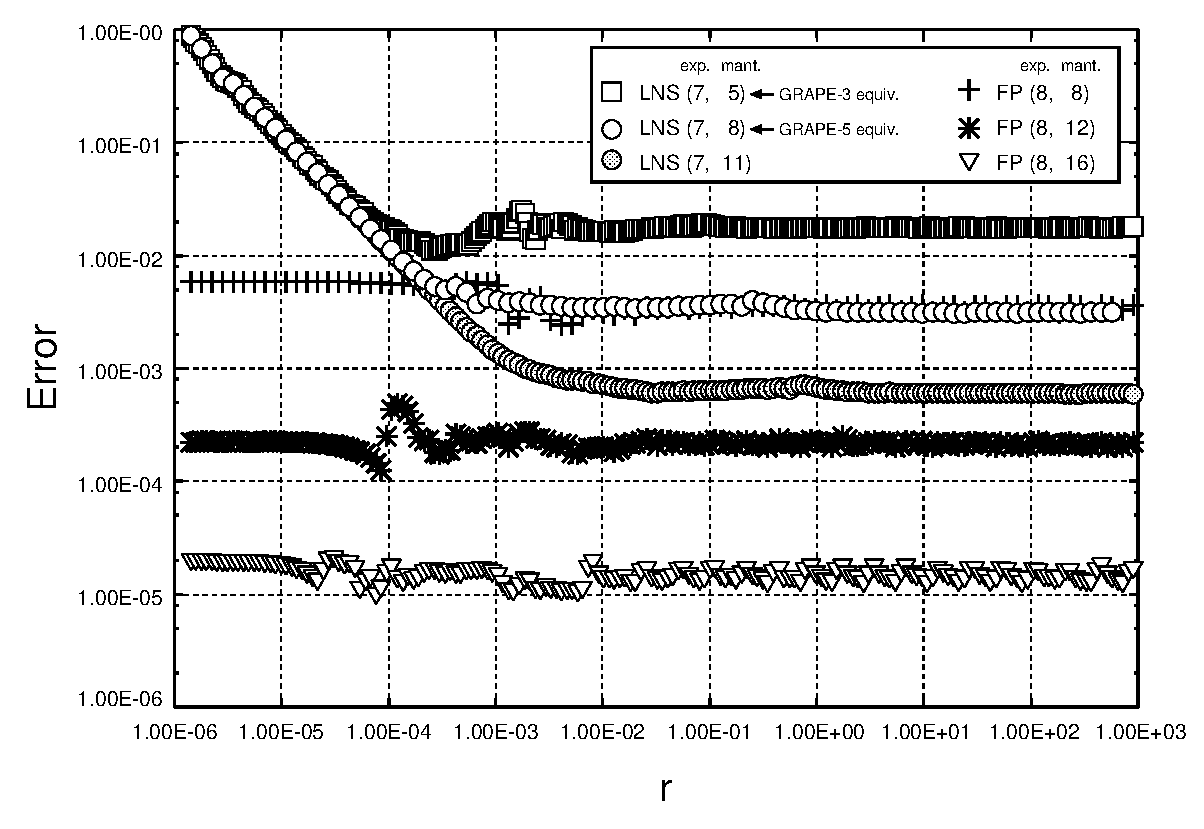
\includegraphics[angle=+0,width=13cm]{./mat/SrGraph.eps}
\caption{Quantization error for froce calculation in the N-body problem.}
\label{SrError}
\end{center}
\end{figure}



\section{Conclusion}
We have developed the PGR package, a software which automatically generate
communication softwares and the hardware descriptions
(the hardware design of pipeline processors)
for FBAs from a high-level description PGDL.
Using the PGR package, we have implemented gravitational force
pipelines used in astrophysical simulations.
The PGDL description for the gravitational force pipelines
is only a several tens of lines of a text file.
Regardless of a very simple description, we could obtain very
efficient implementation. 
Using PGR, we will reach the design area where nobody can achieve.

%------------------------------------------------------------------------- 
\bibliographystyle{latex8}
\begin{thebibliography}{}

\bibitem{AKEDC04}
Azizi, N., Kuon, I., Egier, A., Darabiha, A., \& Chow, P.:
Reconfigurable Molecular Dynamics Simulator.
Proc. of IEEE FCCM'04 Symposium on Field-Programmable Custom Computing Machines, Los Alamitos, CA.
(2004) 197-206

\bibitem{BH98}
Bellows, P., \& Hutchings., B.:
JHDL - An HDL for Reconfigurable Systems.
Proc. of IEEE FCCM'03 Symposium on Field-Programmable Custom Computing Machines, Los Alamitos, CA.
(1998) 175--184

\bibitem{FO01}
Flynn, J., M., \& Oberman, F., S.,:
Advanced Computer Arithmetic Design.
John Wiley \& Sons, New York.
(2001)

\bibitem{GKMK96}
Gokhale, M., Kaba, J., Marks, A., \& Kim, J.:
Malleable architecture generator for FPGA computing.
Proc. SPIE 2914.
(1996) 208--217,

\bibitem{HFKM00}
Hamada,~T., Fukushige,~T., Kawai,~A., \& Makino,~J.:
PROGRAPE-1: A Programmable, Multi-Purpose Computer for Many-Body Simulations.
Publication of Astronomical Society of Japan.
{\bfseries 52} (2000) 943--954

\bibitem{HTYLL03}
Ho, C., Tsoi, K., Yeung, H., Lam, Y., Lee, K., Leong, P., Ludewig, R., Zipf, P., Ortiz, A., \& Glesner, M.:
Arbitrary function approximation in HDLs with application to the n-body problem.
In 2003 IEEE International Conference on Field-Programmable Technology(FPT).
(2003) 84--91

\bibitem{JL01}
Jaenicke, A., \& Luk, A.:
Parametrized Floating-Point Arithmetic on FPGAs.
Proc. of IEEE ICASSP, 
{\bfseries 2} (2001) 897--900

\bibitem{KFMT00}
Kawai,~A., Fukushige,~T., Makino,~J., \& Taiji,~M.:
GRAPE-5: A Special-Purpose Computer for N-body Simulation.
Publication of Astronomical Society of Japan.
{\bfseries 52} (2000) 659--676

\bibitem{LKM02}
Lienhart, G, L., Kugel, A., \& M{\"a}nner, R.:
Using Floating Point Arithmetic on FPGAs to Accelerate Scientific N-Body Simulations.
Proc. of IEEE FCCM'02 Symposium on Field-Programmable Custom Computing Machines, Los Alamitos, CA.
(2002) 182--191

\bibitem{LCCN03}
Leyva, G., Caffarena, G., Carreras, C., \& Nieto-Taladriz, O.:
A Generator of High-speed Floating-point Modules.
Proc. of IEEE FCCM'04 Symposium on Field-Programmable Custom Computing Machines, Los Alamitos, CA.
(2004) 306--307 

\bibitem{LTM03}
Liang, J., Tessier, R., \& Mencer, O.:
Floating Point Unit Generation and Evaluation for FPGAs.
Proc. of IEEE FCCM'03 Symposium on Field-Programmable Custom Computing Machines, Los Alamitos, CA.
(2003) 185--194

\bibitem{MMF97}
Mencer, O., Morf, M. \& Flynn, J., M.:
PAM-Blox: High Performance FPGA Design for Adaptive Computing.
Proc. of IEEE FCCM'98 Symposium on Field-Programmable Custom Computing Machines, Los Alamitos, CA.
(1997) 167--174

\bibitem{M97}
Muller, M., J.:
Elementary Functions: Algorithms and Implementation.
Brikhauser Verlag AG.
(1997)

%% \bibitem{MIE90}
%% Makino, J., Ito, T., \& Ebisuzaki, T.:
%% Error Analysis of the GRAPE-1 Special-Purpose N-Body Machine.
%% Publication of Astronomical Society of Japan.
%% {\bfseries 42} (1990) 717--736

\bibitem{MT98}
Makino,~J., \& Taiji,~M.:
Scientific Simulations with Special-Purpose Computers --- The GRAPE Systems.
Chichester: John Wiley and Sons.
(1998)

\bibitem{MPMF01}
Mencer, O., Platzner, M., Morf, M. \& Flynn, J., M.:
Object-Oriented Domain-Specific Compilers for Programming FPGAs.
IEEE Trans. on VLSI, special issue on Reconfigurable Computing.
(2001)


\bibitem{OMEFS93}
Okumura, K., S., Makino, J., Ebisuzaki, T. Fukushige, T., Ito, T. \& Sugimoto, D.:
Highly Parallelized Special-Purpose Computer, GRAPE-3.
Publication of Astronomical Society of Japan.
{\bfseries 45} (1993) 329--338


\bibitem{SS99}
Stine, J., \& Schulte, M.:
The symmetric table addition method for accurate function approximation.
In Journal of VLSI Signal Processing.
(1999) 167--177

\bibitem{SS03}
Smith, W., D., \& Schore, A., R.:
Towards an RCC-based accelerator for computational fluid dynamics applications.
Proc. of the 2003 International Conference on Engineering Reconfigurable Systems and Algorithms.
(2003)

\bibitem{THYL04}
Tsoi, K., Ho, C., Yeung, H., \& Leong, P.:
An Arithmetic Library and its Application to the N-body Problem.
Proc. of IEEE Symposium on Field-Programmable Custom Computing Machines, IEEE Computer Society Press.
(2004) 68--78

\bibitem{WN04}
Wang, X.,\& Nelson, B., E.:
Tradeoffs of Designing Floating-Point Division and Square Root on Virtex FPGAs
Proc. of IEEE FCCM'03 Symposium on Field-Programmable Custom Computing Machines, Los Alamitos, CA.
(2004) 195--203


\end{thebibliography}

\end{document}
